\chapter{Hot electron temperature modelling}
\label{ch:models-impl}

In this chapter, we will present models of the hot electron absorption trained on the dataset discussed in the previous chapter. The models will be compared and we will also discuss how well the best model represents the behaviour of $T_{\mathrm{hot}}$ compared to other studies. We will also present a simple graphing UI tool which allows to load any supported model and plot the predictions in any axis.

We do not implement the models ourselves, but rather we use optimized open-source libraries that offer rich possibilities of configuration. We will compare the models with each other using mostly \textit{RMSE} metric and $R^2$ statistic. We do not claim that all three models are exhaustingly optimized. We also do not claim that the model we label as best is the only correct solution. The goal of this chapter is to show, how the models work in practice, what are their strengths an weaknesses in this application and what can maybe done in the future to improve them.

We found that the models perform poorly if the data is not transformed. Transforming data is a common step before training a machine learning model. We decided to scale all three parameters to a closed interval [0,1] ($L$ and $I$ logarithmically). If one would skip this step, in SVR and GP, the problem quickly arises because of the absolute value of the distance between two data points needed for the kernel function. For example, if the intensity scale is $10^{17} - 10^{19}$ and scale of angles is $0-60$, the dataset is too sparse for these models to learn the relationship because the distance in the intensity dimension is unproportionally bigger. Moreover, in the parameter space, the distance between $10^{17}$ and $10^{18}$ is roughly ten times smaller than distance between $10^{18}$ and $10^{19}$. The logarithmic transformation is a justified data manipulation based on the visual inspection and the expected nature of the modelled relationship.

In the actual implementation, the classes which represent all three models follow an abstract structure that allows us to work with different models flexibly. For example, the instance of a transformer class used in the training is saved to a member variable of the model class. In general, the parameters of the transformer can differ for different models. Also, after training using transformation the data have to be transformed in the same way before the prediction as well.

For each model, we will now provide a brief introduction regarding the implementation. Then we compare the performance of these models using 8-fold cross-validation. In the end, we also compare the models by visual inspection of the prediction graphs sampled on for the same parameters as in the presentation of the dataset.

\section{Models}
\label{sec:temp-models}

For training the SVR model we used \textit{SVR} class from Python \textit{scikit-learn} library. For kernel we selected the RBF kernel. There are multiple hyper-parameters to be optimized - $\epsilon$ and $C$ from SVR itself and $\gamma$ from the RBF kernel which is here defined as $\mathrm{RBF}(\bm{x},\bm{x^\prime}) = \mathrm{exp}(\gamma \norm{\bm{x}-\bm{x^\prime}})$. During the cross-validation, where we calculate \textit{RMSE} and $R^2$ on test set for each fold, the hyper-parameters are selected via grid-search using an additional cross-validation on the training set.

The neural network model was trained using the \textit{PyTorch} library in Python. The architecture is a fully-connected neural network with two hidden layers, each containing 64 neurons with \textit{ELU} activation functions. A dropout rate of 0.2 and a weight decay of $0.1$ were applied to compensate the over-parametrization. The model was optimized using the \textit{Adam} optimizer over 2500 epochs with a learning rate of 0.02 minimizing the \textit{MSE} loss function. These hyper-parameters were chosen based on multiple attempts to find a good NN model.

Gaussian processes regression was done using \textit{GPRegression} from \textit{GPy} library also in Python. \textit{GPy} is a very robust and numerically stable tool for Gaussian process regression and classification. We used the \textit{Mattern} kernel defined by \ref{eq:mattern-kernel} with $\nu = 3/2$. The hyper-parameters are $\sigma$ (observation noise), $\sigma_k^2$ (kernel variance) and $l$ (kernel scale). The GPy class \textit{GPy.models.GPRegression} has its own optimizer, which can find the optimal hyper-parameters using maximum likelihood approach very effectively. 

\subsection*{K-Fold crossvalidation of the models}
\begin{table}[h]
	\centering
	\caption{Cross-validation of SVR, NN and GP models.} 
	\begin{tabular}{ c c c c c c c }
		\toprule
		\  & $SVR_\mathrm{rmse}$& $SVR_\mathrm{r2}$ & $NN_\mathrm{rmse}$   & $NN_\mathrm{r2}$ & $GP_\mathrm{rmse}$ & $GP_\mathrm{r2}$ \\ 
		\midrule
		Fold 1 & 35.13 & 0.96 & 30.97 & 0.97 & 27.55 & 0.98 \\ 
		Fold 2 & 47.61 & 0.93 & 40.82 & 0.95 & 37.28 & 0.96 \\ 
		Fold 3 & 33.18 & 0.98 & 31.51 & 0.98 & 23.94 & 0.99 \\ 
		Fold 4 & 79.91 & 0.90 & 43.35 & 0.97 & 40.80 & 0.97 \\ 
		Fold 5 & 36.95 & 0.97 & 30.09 & 0.98 & 31.05 & 0.98 \\ 
		Fold 6 & 69.68 & 0.90 & 43.04 & 0.96 & 37.00 & 0.97 \\ 
		Fold 7 & 41.01 & 0.95 & 37.71 & 0.96 & 33.78 & 0.97 \\ 
		Fold 8 & 60.28 & 0.94 & 41.18 & 0.97 & 38.96 & 0.97 \\ 
		\midrule
		Mean & 50.47 & & 37.33 & & 33.80 & \\ 
		\bottomrule
	\end{tabular}
	\label{tab:cross-val} 
\end{table}

For all three selected models, we performed an 8-fold cross-validation. This approach allows for a robust and reliable comparison between the models. For each fold, we calculated the root mean square error (RMSE) and the $R^2$ statistic on the test data. The detailed results for each fold, along with the mean values, are presented in Table \ref{tab:cross-val}.

As shown in the table, the mean square errors are of the same order for all three models. Some folds tend to produce worse results in general, which is expected. Specifically, it is guaranteed that in one of the folds, the dataset's minimum or maximum value might be missing from the training set. This can result in a higher RMSE due to such an \textit{unlucky} division. This is precisely why we perform 8-fold cross-validation, as on average, these random factors cancel out. The high values of $R^2$ hint that the models are able to capture the modeled relationship at least roughly. The SVR model demonstrates the worst predictive performance. In contrast, the NN and GP models exhibit similar results, though the NN is better only in fold 5. These two models will be compared in greater detail in the following sections.


\subsection*{Neural Network model}
The predictions of NN model trained with the same technique as before but now on the whole dataset can be seen in the figure \ref{fig:nn-pred}. The parameter space is the same as in previous chapter when we were presenting the dataset. Now we increased the density by which the model is sampled to grid 50 by 50 (also logarithmic in $L$ axis).
\begin{figure}[ht]
	\centering
	\begin{subfigure}{0.49\textwidth}
		\centering
		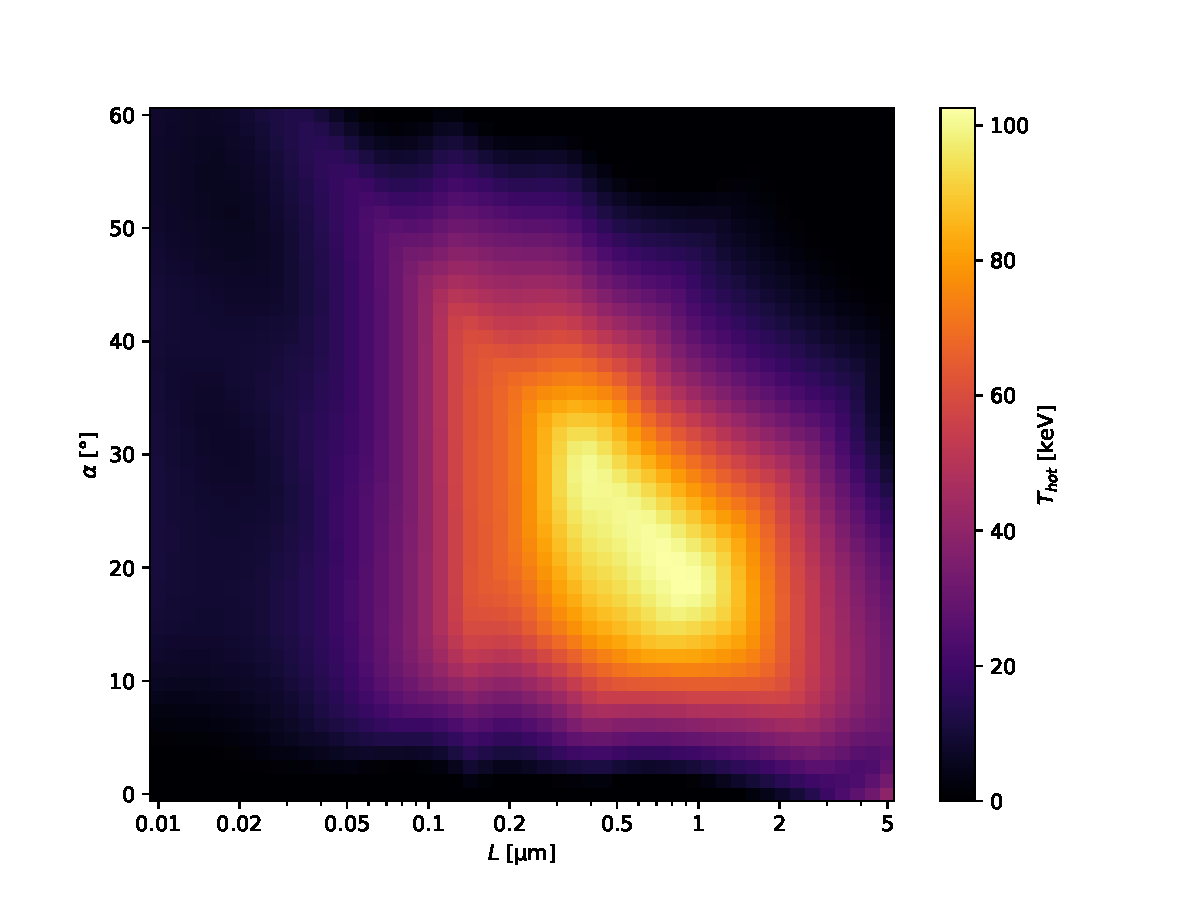
\includegraphics[width=\textwidth]{figures/nn17_pred}
		\caption{Predictions of NN model for $I = 1 \times 10^{17} \, \mathrm{W.cm}^{-2}$.}
		\label{fig:nn-pred-a}
	\end{subfigure}
	\hfill
	\begin{subfigure}{0.49\textwidth}
		\centering
		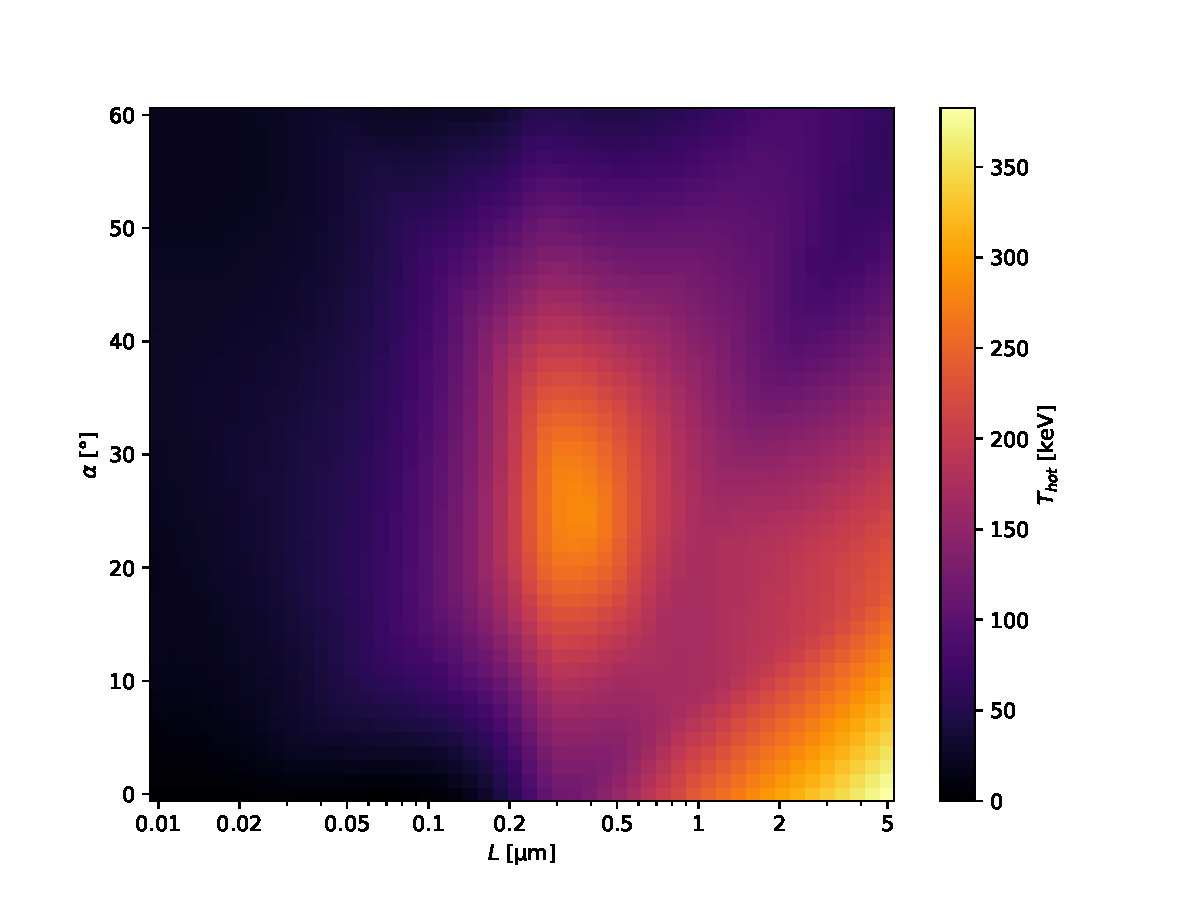
\includegraphics[width=\textwidth]{figures/nn18_pred}
		\caption{Predictions of NN model for $I = 1 \times 10^{18} \, \mathrm{W.cm}^{-2}$.}
		\label{fig:nn-pred-b}
	\end{subfigure}
	\begin{subfigure}{0.59\textwidth}
		\centering
		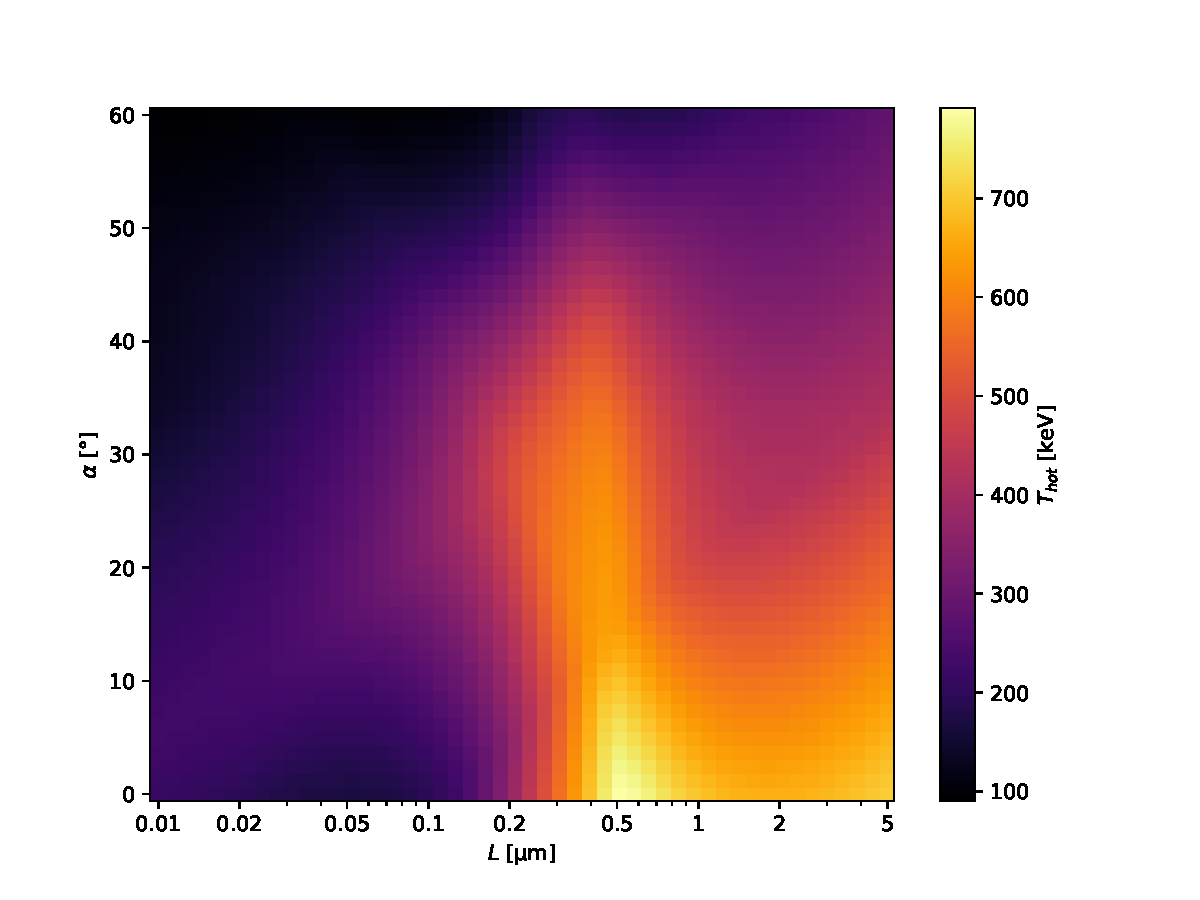
\includegraphics[width=\textwidth]{figures/nn19_pred}
		\caption{Predictions of NN model for $I = 1 \times 10^{19} \, \mathrm{W.cm}^{-2}$.}
		\label{fig:nn-pred-c}
	\end{subfigure}
	\caption{Predictions of NN model.}
	\label{fig:nn-pred}
\end{figure}

With the NN model, achieving smoothness is quite challenging because the fitting process does not explicitly account for the relationship between two data points. Regularization techniques such as weight decay and dropout do provide some improvement, though likely not as much as desired. The presence of sharp lines or ridges in the graphs indicates that the model does not generalize the relationships well enough. While further regularization could potentially increase smoothness, the results seen in the prediction graphs are probably expected given the small size of the dataset.

Despite these issues, the maxima appear to be in the correct parameter regions, and the maximum hot electron temperature is reasonably consistent with the values present in the dataset. However, it is important to note that the neural network can produce negative predictions, which do not have any physical interpretation. To address this, we decided to convert all negative predictions to zero.

Generally, it is possible to claim that the over-parametrized model can be smoothened to acceptable condition. However, it is still not completely clear, whether this architecture can capture the true physical relationship or not. The ridges, which are visible for predictions with $I = 10^{11} \, \mathrm{W.cm}^{-2}$ suggest either that we need more data, or that the total number of neurons is a little low.


\subsection*{Gaussian process regression model}

\begin{figure}[ht]
	\centering
	\begin{subfigure}{0.49\textwidth}
		\centering
		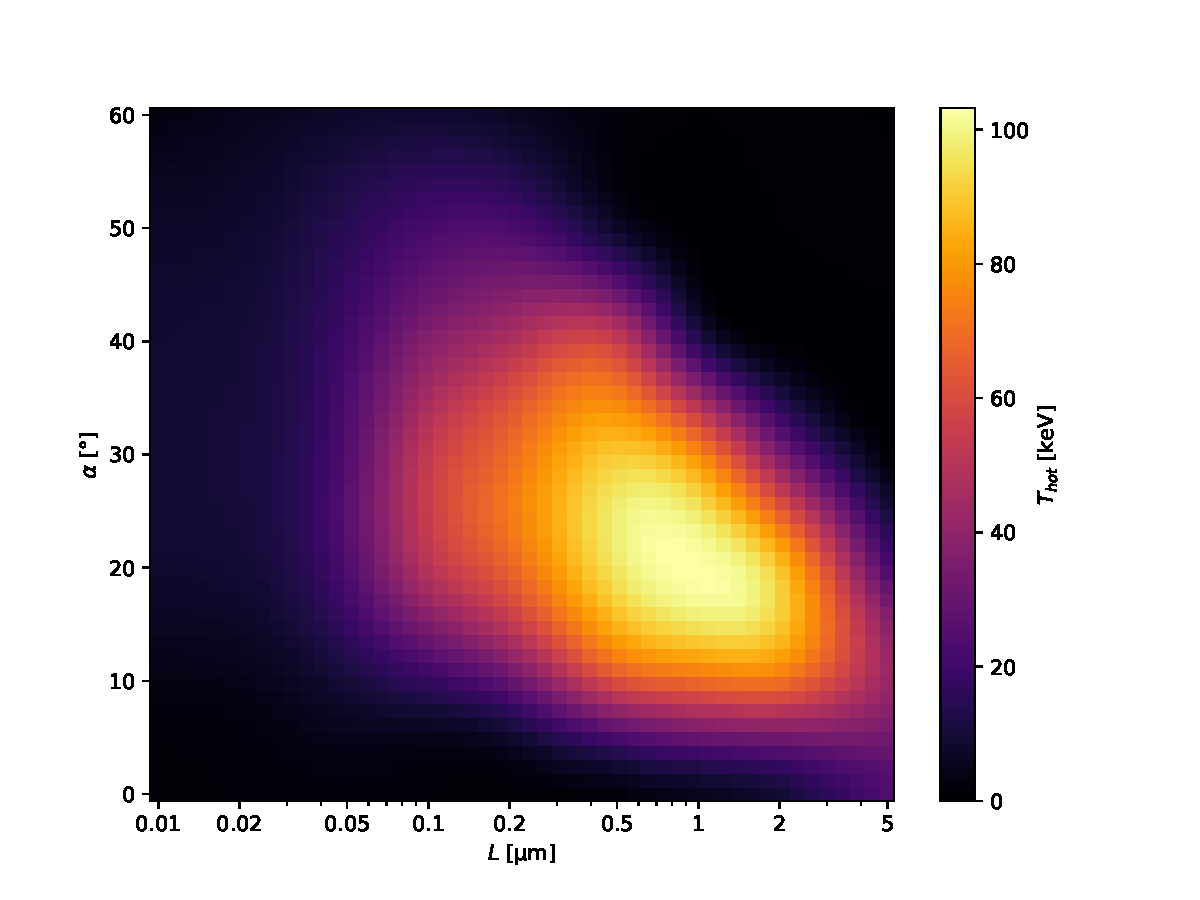
\includegraphics[width=\textwidth]{figures/gp17_pred}
		\caption{Predictions of GP model for $I = 1 \times 10^{17} \, \mathrm{W.cm}^{-2}$.}
		\label{fig:gp-pred-a}
	\end{subfigure}
	\hfill
	\begin{subfigure}{0.49\textwidth}
		\centering
		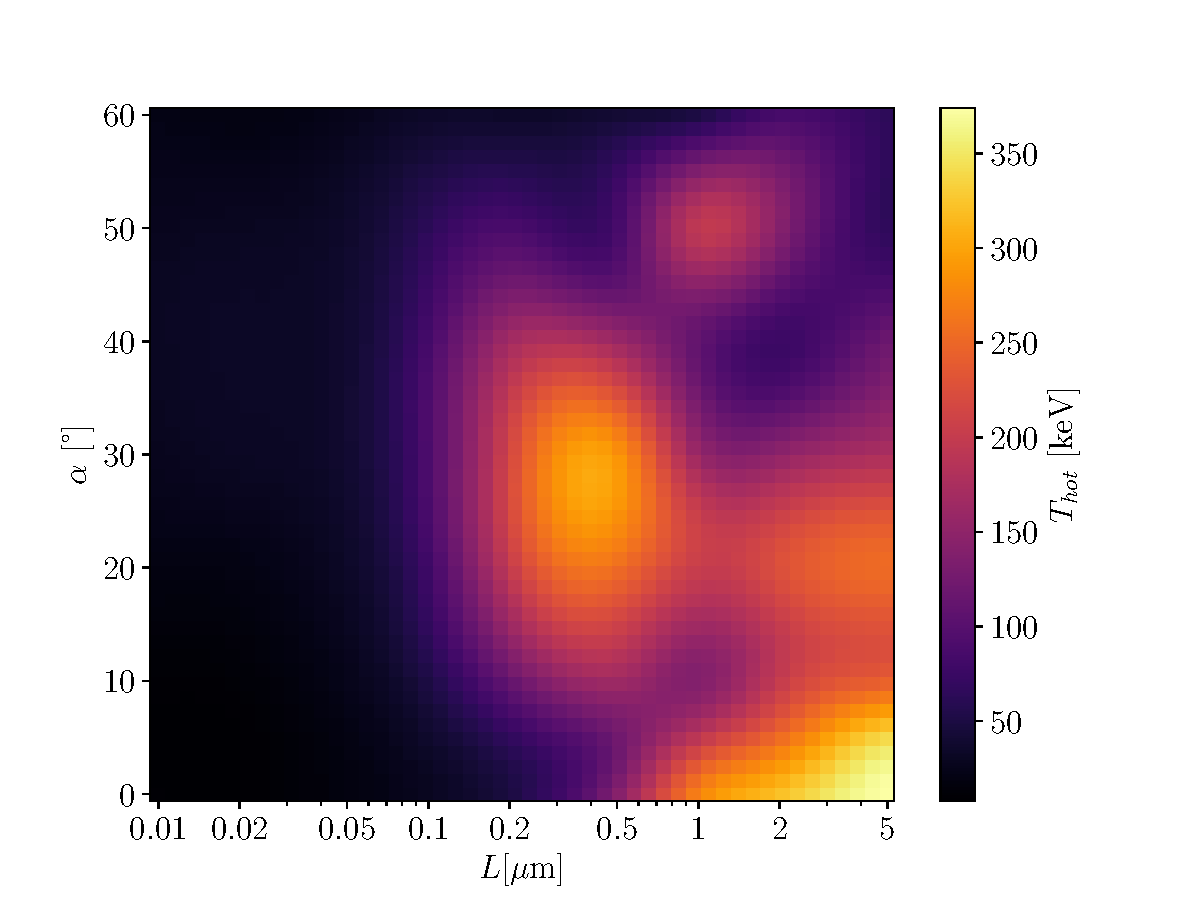
\includegraphics[width=\textwidth]{figures/gp18_pred}
		\caption{Predictions of GP model for $I = 1 \times 10^{18} \, \mathrm{W.cm}^{-2}$.}
		\label{fig:gp-pred-b}
	\end{subfigure}
	\begin{subfigure}{0.49\textwidth}
		\centering
		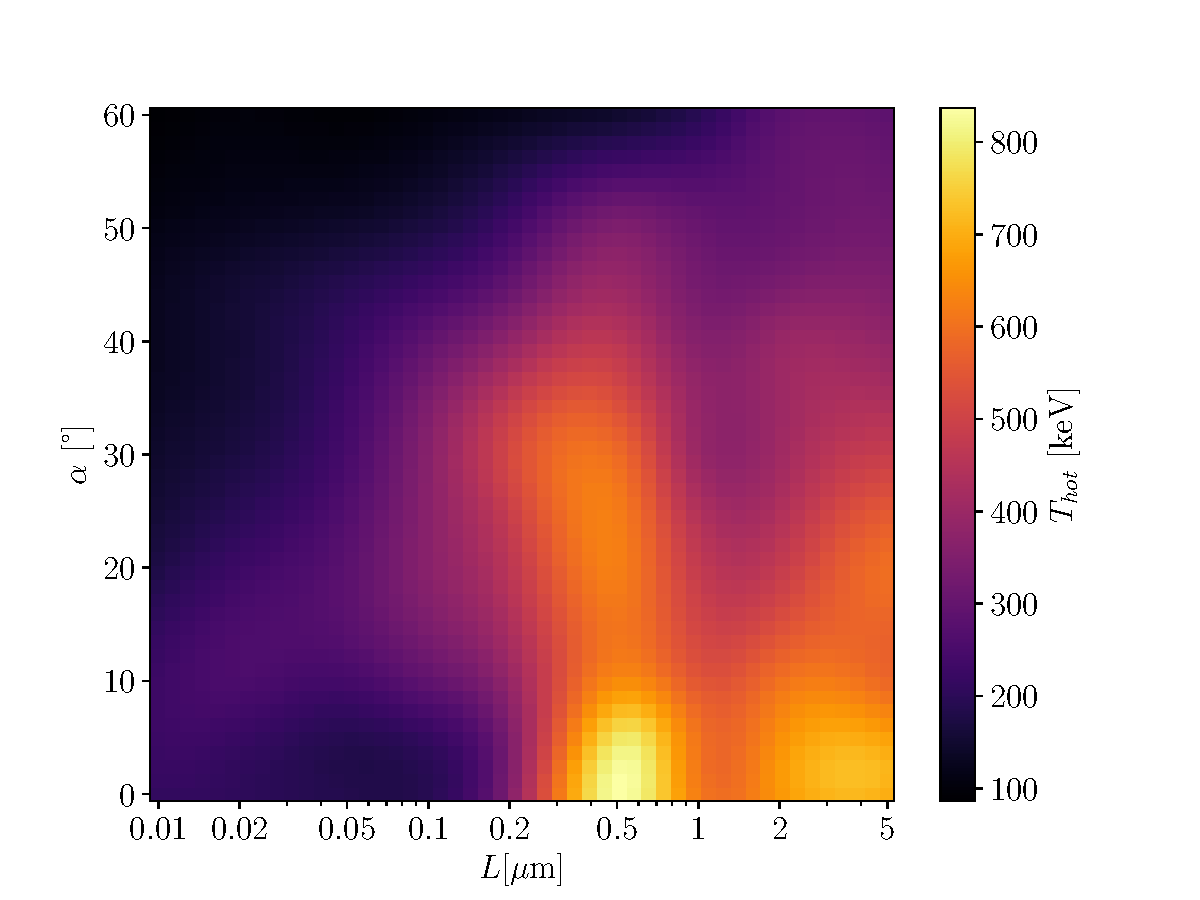
\includegraphics[width=\textwidth]{figures/gp19_pred}
		\caption{Predictions of GP model for $I = 1 \times 10^{19} \, \mathrm{W.cm}^{-2}$.}
		\label{fig:gp-pred-c}
	\end{subfigure}
	\caption{Predictions of the GP model.}
	\label{fig:gp-pred}
\end{figure}

The GP regression model has shown the best performance on the cross-validation test. Let us remind, that once the optimal parameters of the kernel are found, the predictions are calculated from the posterior distribution as it was presented in section \ref{sec:gp-theory}. The kernel parameters optimized on the whole dataset are $\sigma_k^2 =29179.49$, $l = 0.36$ and $\sigma^2 = 665.06$. The predictions shown in similar way as for NN model can be seen in figure \ref{fig:gp-pred}.

Immediately one can see, that these predictions are much smoother than those of NN model although in general, they are very similar. Probably the biggest qualitative difference can be found in the predictions for $I = 1 \times 10^{19} \, \mathrm{W.cm}^{-2}$, where the maximum temperature is lower for NN, whereas in GP the peak has almost exactly the same value as the dataset. Also, in graph for $I = 1 \times 10^{18} \, \mathrm{W.cm}^{-2}$, there is a local maximum for $\alpha = 50\degree$ and $L \approx 1 \, \mu\mathrm{m}$, which cannot be observed in the predictions of NN model.

\begin{figure}[ht]
	\centering
	\begin{subfigure}{0.49\textwidth}
		\centering
		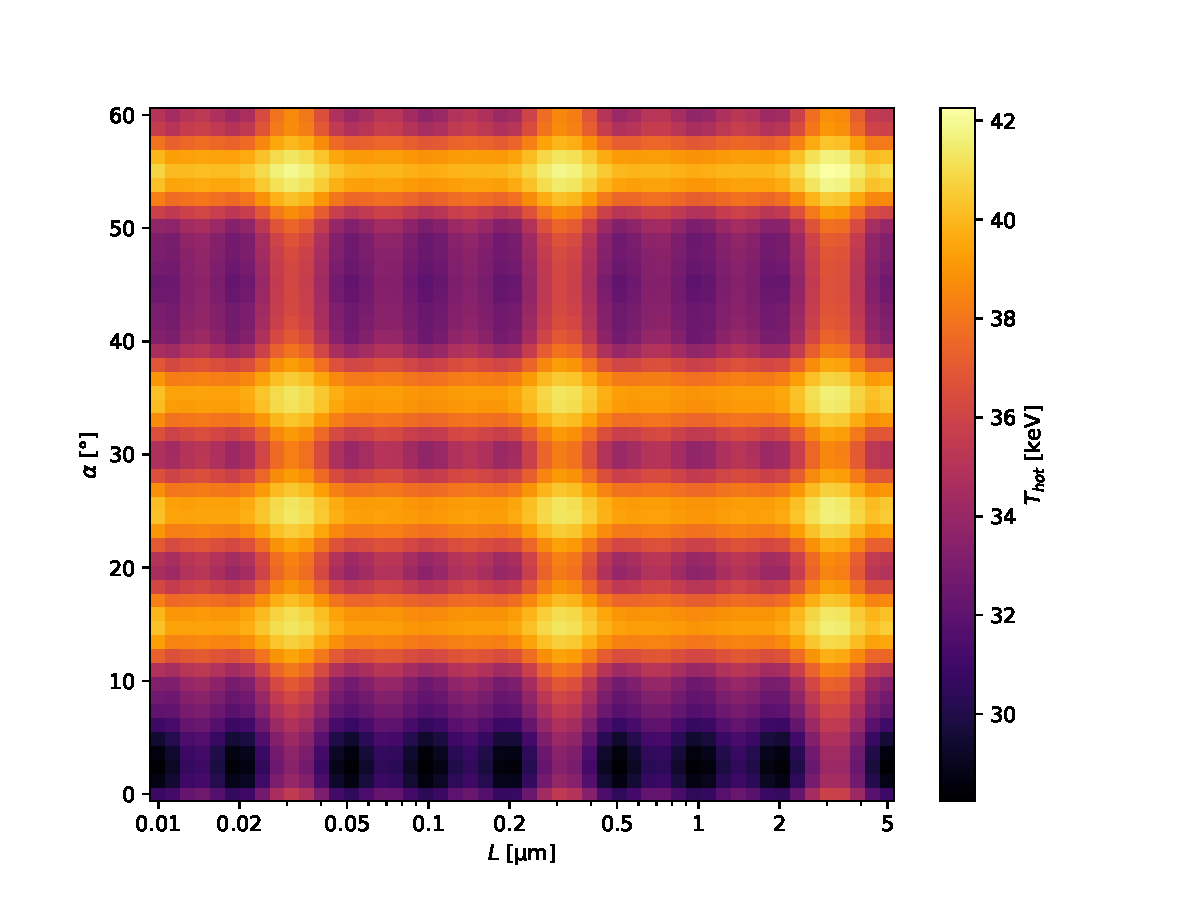
\includegraphics[width=\textwidth]{figures/gp17_pred_ss}
		\caption{Uncertainty of GP model for $I = 1 \times 10^{17} \, \mathrm{W.cm}^{-2}$.}
		\label{fig:gp-pred-ss-a}
	\end{subfigure}
	\hfill
	\begin{subfigure}{0.49\textwidth}
		\centering
		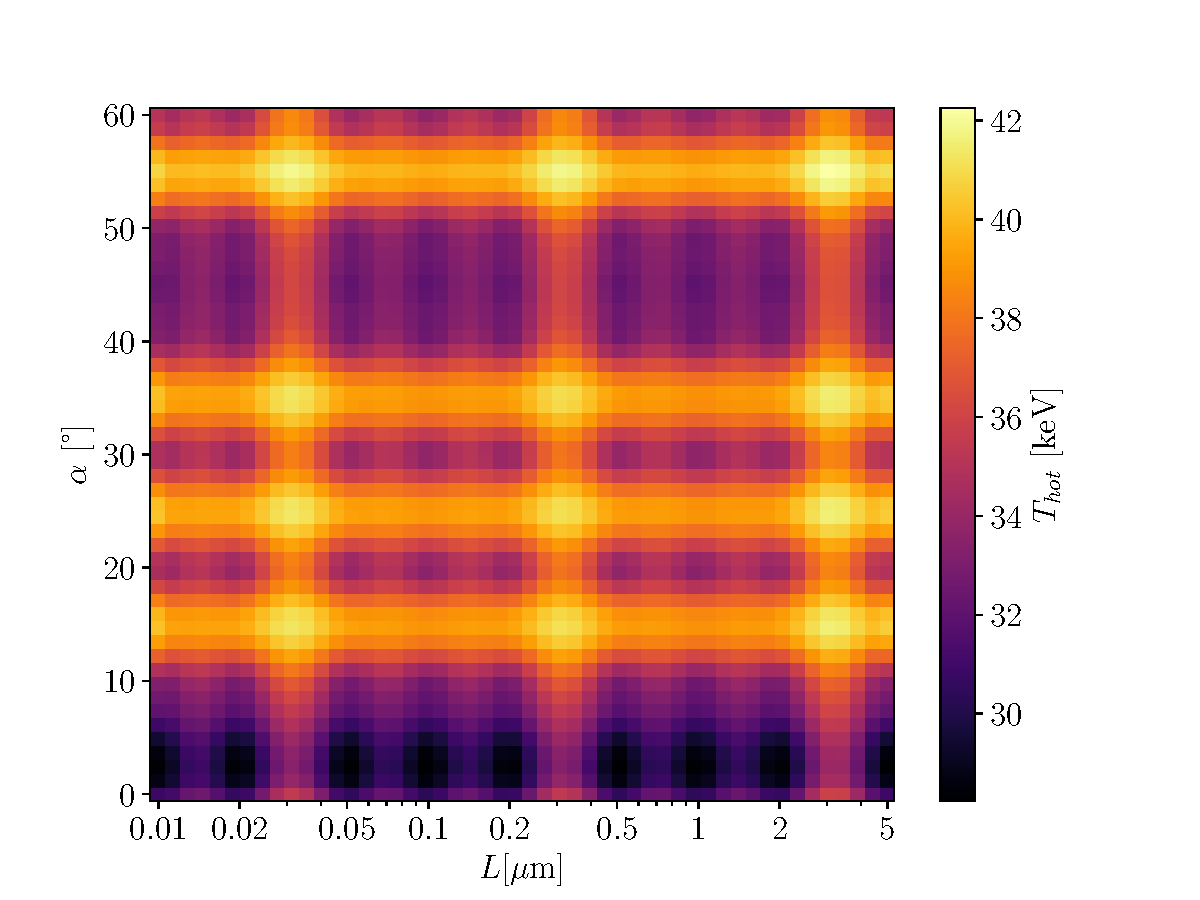
\includegraphics[width=\textwidth]{figures/gp18_pred_ss}
		\caption{Uncertainty of GP model for $I = 1 \times 10^{18} \, \mathrm{W.cm}^{-2}$.}
		\label{fig:gp-pred-ss-b}
	\end{subfigure}
	\begin{subfigure}{0.49\textwidth}
		\centering
		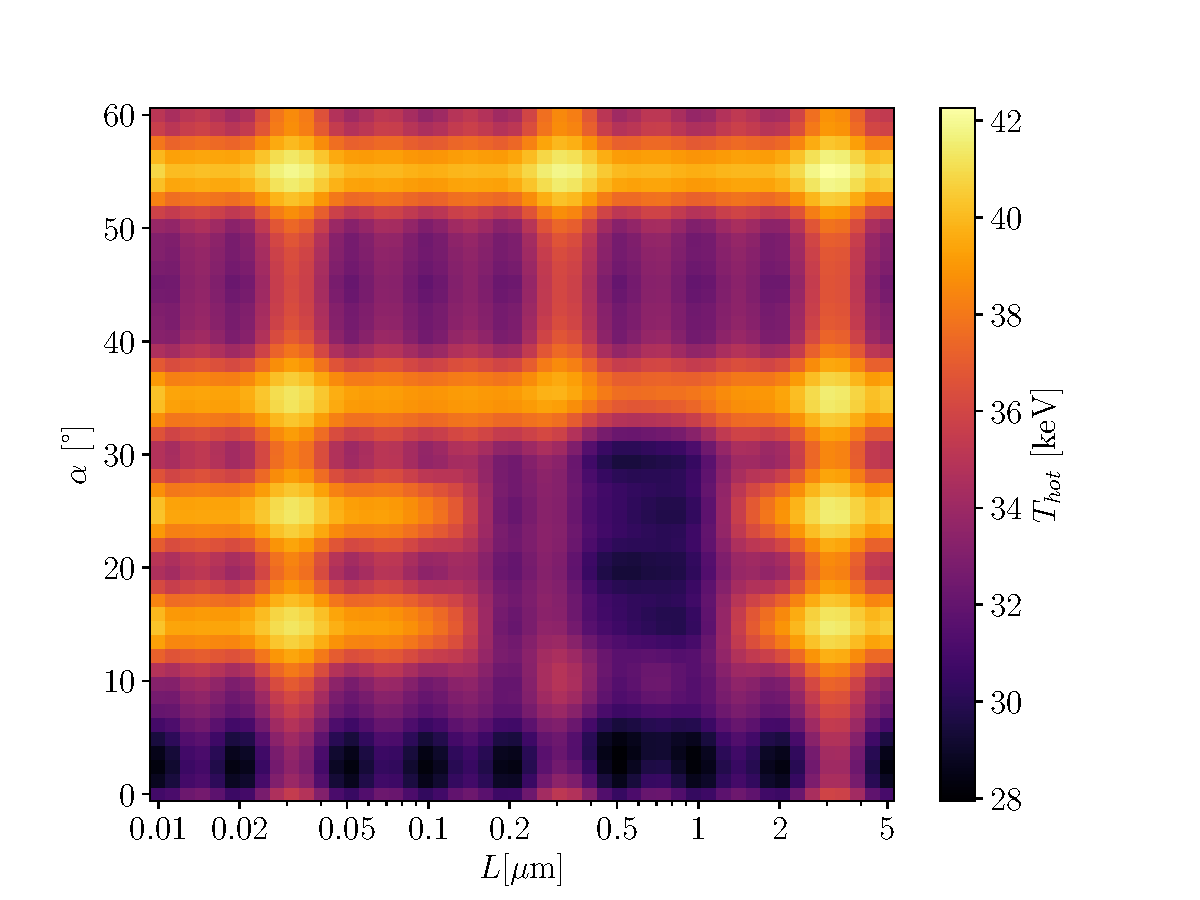
\includegraphics[width=\textwidth]{figures/gp19_pred_ss}
		\caption{Uncertainty of GP model for $I = 1 \times 10^{19} \, \mathrm{W.cm}^{-2}$.}
		\label{fig:gp-pred-ss-c}
	\end{subfigure}
	\caption{Uncertainty of the GP model.}
	\label{fig:gp-pred-ss}
\end{figure}

Now let us come back to one of the biggest strengths of the GP model. As it was stated in the section \ref{sec:gp-theory}, the GP model consists of mean function and covariance function. The predictions in \ref{fig:gp-pred} are the mean evaluated in given points. The variance of these points is calculated as diagonal elements of a matrix corresponding to the covariance function in the testing points. These values are scaled with optimized parameter of GP - noise variance $\sigma^2$. The interpretation of this parameter is therefore straightforward.

It is possible to create same plots but for the standard error $\sigma$. Such plots are shown in the figure \ref{fig:gp-pred-ss}. Naturally, the uncertainty is smaller where the training data is denser and larger in areas with sparse data. The denser the dataset, the smaller the error. The dataset was primarily created using a grid distribution of the simulation parameters. The plots hint that the dataset is denser for small angles (up to 10°), which is true. Additionally, there is a higher density of data for the intensity $I = 10^{17} \, \mathrm{W.cm}^{-2}$ around $L = 0.5\mu \mathrm{m}$ and for $\alpha$ in range of $15\degree$ to $ 30\degree$, as confirmed by the graphs.

\section{Prediction UI tool}
For the purpose of visual comparison of the models, another tool was developed. The main goal is to allow user to be able to look at the predictions of different models in different axes than those which we used until now. Plotting of custom looks can be tedious if one is writing each time a new script. Also, working with 4 dimensional data is unpleasant, because it is not possible to draw everything in one graph without sacrificing readability.

The tool provides an user interface for several basic options that are relevant for this analysis and a graph of the predictions based on the configuration. A screenshot from this application is shown in the figure \ref{fig:graph-tool}.

\begin{figure}[h]
	\centering
	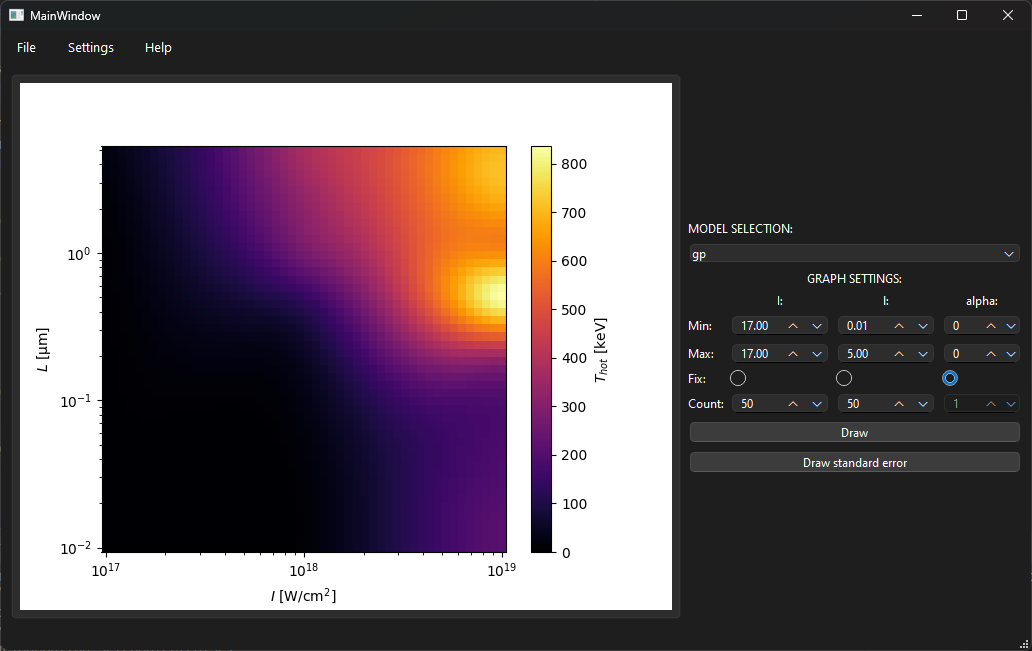
\includegraphics[width=0.85 \textwidth]{figures/graph_tool}
	\caption{A screenshot from the graphing tool with graph of GP model for $\alpha = 0\degree$.}
	\label{fig:graph-tool}
\end{figure}

The tool is quite simple, but it is tailored for this application, so it almost exhaustingly fulfils the need for special tool. It might be useful even beyond the scope of this thesis for example if someone decides to improve the models we presented or if he just wants to inspect them more closely. 

The application is implemented in Python in \textit{PyQt6} framework with the additional use of class \textit{FigureCanvasQTAgg} from \textit{matplotlib} library. The core of the functionality is relying on an abstraction, where the models are represented as a class with particular members - functions \textit{load} and \textit{predict} and already mentioned member variable of custom type \textit{Transformer}. There are also few more classes which make it easier to work with the prediction grid and the graphing canvas. Adding a support for more, completely different models is only a matter few lines of code as long s the abstraction is followed. Currently only NN, SVR and GP are supported.

\begin{figure}[h]
	\centering
	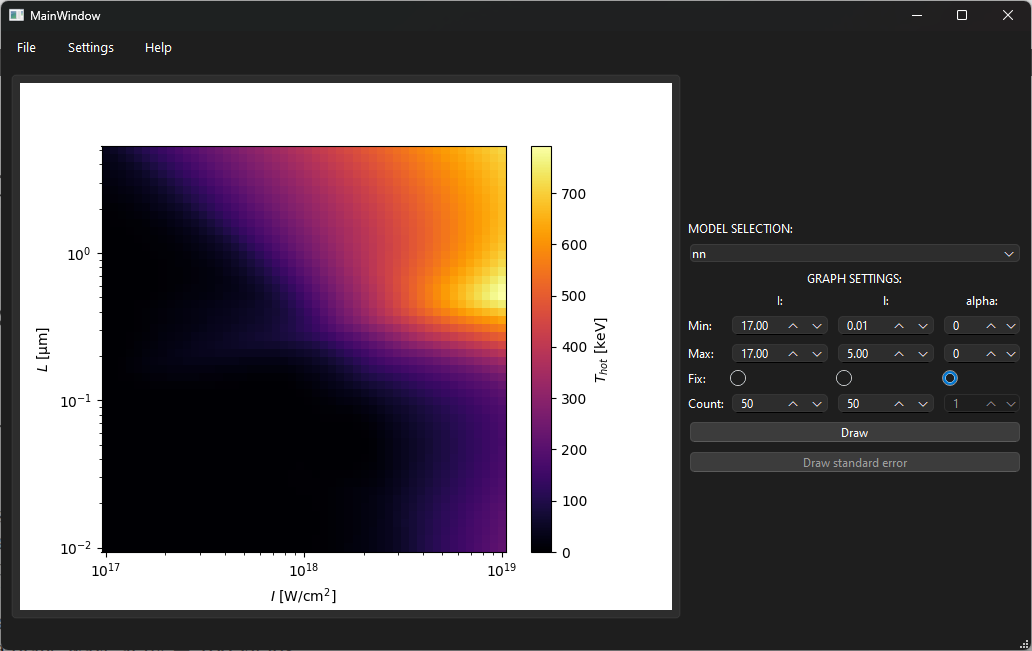
\includegraphics[width=0.85 \textwidth]{figures/graph_tool2}
	\caption{A screenshot from the graphing tool with graph of NN model for $\alpha = 0\degree$.}
	\label{fig:graph-tool2}
\end{figure}


After choosing a model, the user can choose, which axis he wants to \textit{fix} and at which value. Before, we were always fixing the intensity to three values and sampled $L$ and $\alpha$. Then, the user chooses the ranges (\textit{min}, \textit{max}) of the remaining two axes alongside with the density of the sample (\textit{count}). Prediction of the same configuration as before but for NN model is shown in the figure \ref{fig:graph-tool2}. In both examples, notice the smooth transition between the intensities. Remember that there are almost no training point off the three intensities, so the predicted temperatures could not be very accurate.

Drawing of the error is currently supported only for the GP model. By clicking the \textit{Draw standard error} button the prediction standard error is drawn. The screenshot with standard error can be seen in figure \ref{fig:graph-tool3}.

\begin{figure}[h]
	\centering
	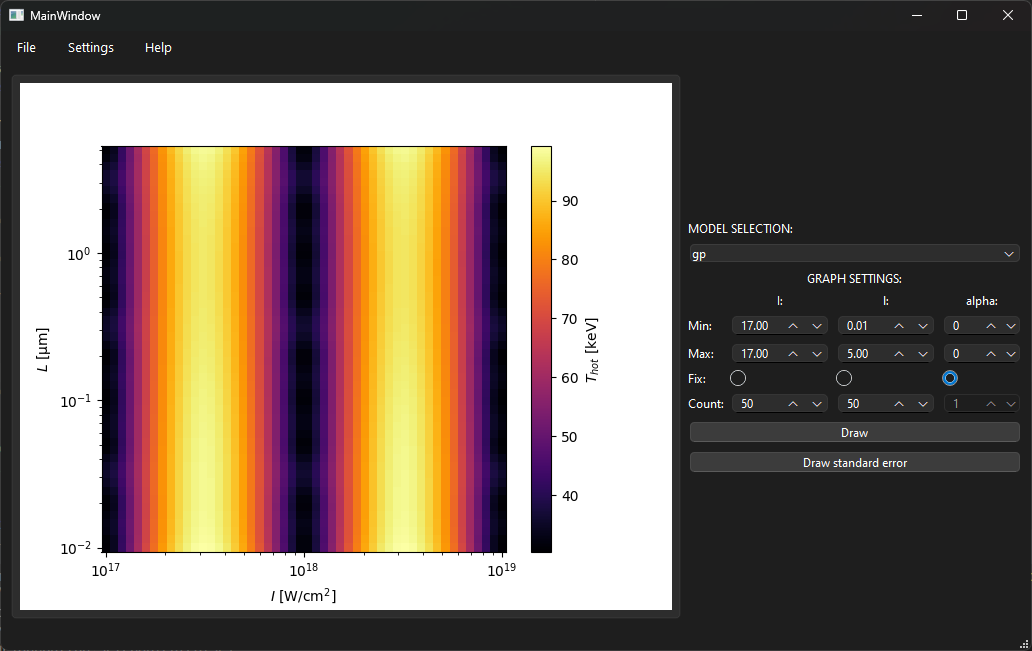
\includegraphics[width=0.85 \textwidth]{figures/graph_tool3}
	\caption{A screenshot from the graphing tool with graph of standard error of GP model for $\alpha = 0\degree$.}
	\label{fig:graph-tool3}
\end{figure}

After previous discussion, it shouldn't surprise us that the uncertainty is larger for intensities that are not a power of 10. Similar error pattern is visible when $L$ is the fixed axis, instead of $\alpha$.



\section{Comparison to other temperature scaling}
\label{ch:comparison}
In this last section, the models are compared to a few of the previous works which studied the scaling of hot electron temperature.

First, the comparison will be done with respect to work of \textit{Cui et al.}\cite{cui2013}, where they model scaling of hot electron temperature with intensity as: 
\begin{equation}
	\label{eq:cui-scale}
	T_{\mathrm{hot}} = \left(\frac{I\lambda^2}{10^{18} \, W \, \mathrm{cm}^{-2} \, \mathrm{\mu m}^2}\right)^{1/3} \times 1.01 \, \mathrm{MeV},
\end{equation}
which, as they have shown, approximately holds for the optimized scale length and angle of resonance absorption ($\lambda = 1$ and $\alpha = 21.6$) given by \ref{eq:res-opt}.

The GP model trained by us gives predictions that can be seen in the figure \ref{fig:cui-compare-1}.

\begin{figure}[h]
	\centering
	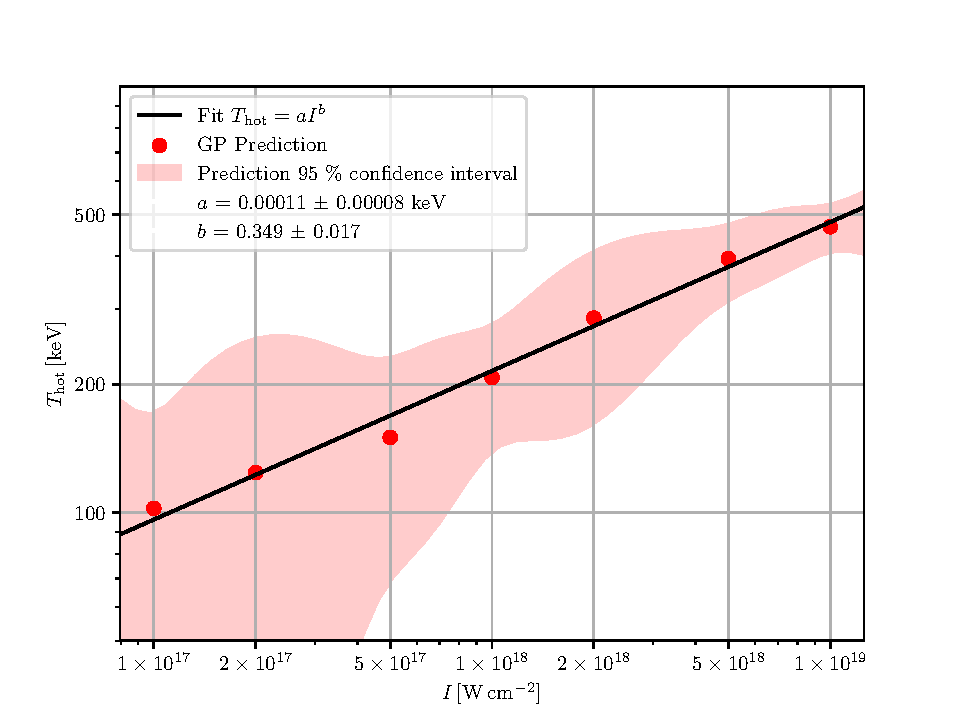
\includegraphics[width=0.95 \textwidth]{figures/cui_compare1}
	\caption{The predictions of GP model for optimized resonance absorption $\lambda = 1$ and $\alpha = 21.6 \degree$. The equation of the fit as well as the fitted parameters is shown in the legend. The red area depicts the 95\% confidence interval of the predictions.}
	\label{fig:cui-compare-1}
\end{figure}

After fitting the predictions of the GP model with a function $T_{\mathrm{hot}}= aI^b$, we get the estimates $a=0.00012\pm0.00008 \, \mathrm{keV}$ and $b=0.349\pm0.017$. The fitted curve is a straight line in the graph because of the choice of scales.

For numerical comparison, the coefficient $a$ has to be scaled with $a^* = a\times 10^6$ because of the unit conversion used bu Cui et al.. This gives us $a^* = 120 keV$ which is still roughly 10 times larger than the constant $1.01\, \mathrm{MeV}$ from equation \ref{eq:cui-scale}. The difference is probably caused by the fact that in \cite{cui2013}, they used hot electron temperatures from the time of interaction. As they show themselves, the temperature drops quite rapidly with time, which would explain why our temperatures are lower.
Other than that, the exponent estimate  $b=0.349\pm0.017$ is within one standard error in a agreement with scaling $T_\mathrm{hot} \sim I^{1/3}$.	

If the angle of incidence is not satisfying the condition \ref{eq:res-opt}, the relationship seems to become more complicated. In \cite{cui2013}, they looked for power coefficient for $T_\mathrm{hot} \approx I^{b}$ at $\lambda = 1$ and $\alpha = 45\degree$ and estimated it as $b=0.64$. They used two datapoints $I = 10^{17} \, W \, \mathrm{cm}^{-2}$ and $I = 10^{19} \, W \, \mathrm{cm}^{-2}$ and for these two points we get similar estimate $b$. However, if we sample the space more densely, our model predicts non-trivial relationship which cannot be easily fitted with simple power function. The predictions  together with function $T_\mathrm{hot} \sim I^{0.64}$ can be seen in figure \ref{fig:cui-compare-2}.

\begin{figure}[h]
	\centering
	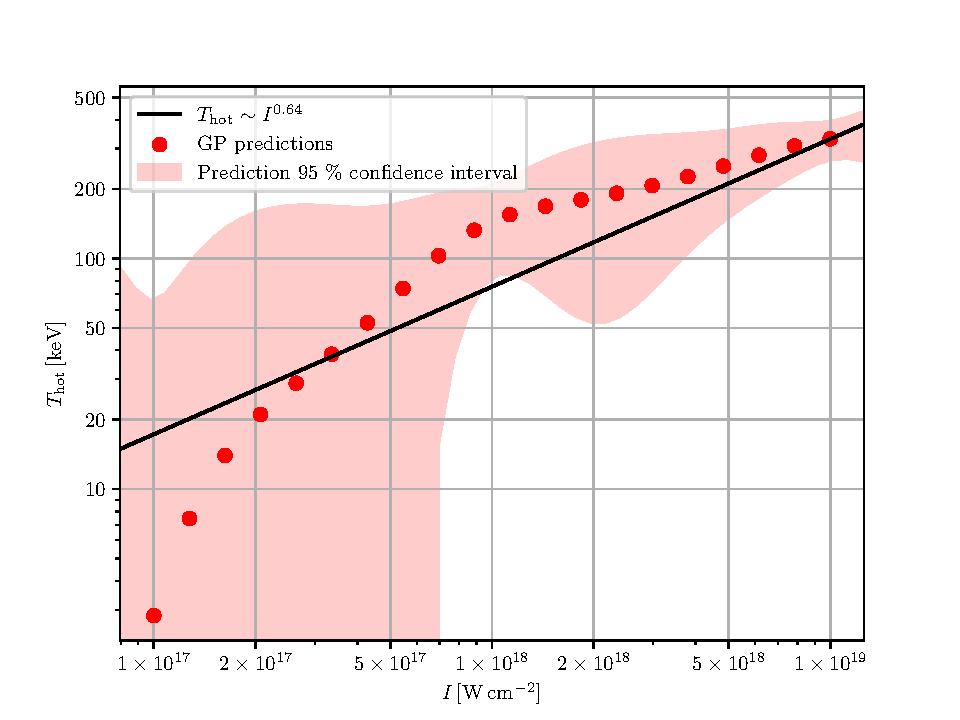
\includegraphics[width=0.95 \textwidth]{figures/cui_compare2}
	\caption{The predictions of GP model for $\lambda = 1$ and $\alpha = 45\degree$. The red area once again shows the 95\% confidence interval of the predictions.}
	\label{fig:cui-compare-2}
\end{figure}

One can note that the predictions for the intensity $I = 10^{18} \, \mathrm{W} \, \mathrm{cm}^{-2}$ do not match the power rule $T_\mathrm{hot} \sim I^{0.64}$. Keep in mind, that the model was mostly trained for three intensities in majority of the grid with few exceptions. It might be interesting that the shape of the predictions in the figure \ref{fig:cui-compare-2} much resemble to other graph (figure 2) from \cite{cui2013}, which depicts \textit{absorption rate} instead of the temperature. 

\section{Strategy for choosing the next simulations}

This section is dedicated to the last unresolved issue of this thesis. We need a strategy for expanding the dataset with the goal of improving the model accuracy. The inherent capability of GP models to provide not only predictions but also an estimate of the uncertainty associated with those predictions makes them well-suited for this task.

The first step in this strategy is to examine the GP model's uncertainty estimates to identify regions with high predictive uncertainty. These regions are typically visualized using standard error plots. Areas with larger uncertainties are prime candidates for further exploration, as additional data from these regions can significantly reduce the overall uncertainty of the model. By focusing on these high-uncertainty regions, we can ensure that resources are used efficiently, targeting the most informative parts of the parameter space.

Once high-uncertainty regions have been identified, the next step is to select specific input parameters within these regions for new simulations. Naturally, resulting data is used to update the GP model. This iterative process is repeated, gradually refining the model and reducing uncertainty across the parameter space.

One of the major strengths of this strategy is its efficient use of resources. By focusing on areas of high uncertainty, we ensure that each new experiment or simulation provides high information gain. Additionally, the GP model's uncertainty estimates are dynamic, allowing for real-time adjustments in the exploration strategy as new data becomes available. 

However, there are also some weaknesses to this strategy. The effectiveness of the approach heavily depends on the initial GP model's ability to reasonably approximate the underlying data distribution. If the initial model is poorly constructed, the uncertainty estimates may be misleading. Additionally, if the original model was constructed using parameters selected from grid, it is likely that the uncertainties will be highest in points from which the training inputs are furthest.

When comparing Figure \ref{fig:graph-tool3} to Figure \ref{fig:gp-pred-ss}, one can see that the uncertainties are much larger for the stripes of unexplored intensities. We performed six simulations with parameters selected from the region of high uncertainties to demonstrate how this strategy works in practice. Results of these simulations can be seen in the table \ref{tab:new-simulations}.

\begin{table}[h]
	\centering
	\caption{Parameters of new simulations.}
	\begin{tabular}{c c c c c}
		\toprule
	     $I \, \left[W \mathrm{cm}^{-2}\right]$ & $L \, \mathrm{[\mu m]}$ & $\alpha \, \mathrm{[\degree]}$  & $T_\mathrm{hot} \, [\mathrm{keV}] $ &  $\Delta T_\mathrm{hot} \, [\mathrm{keV}]$ \\ 
		\midrule
		$5\times 10^{17}$ & 0.01 &0 &3.03 &0.11  \\
		$5\times 10^{17}$ & 1.00 &0 &80.55 & 15.89 \\
		$5\times 10^{17}$ & 5.00 &0 &212.01 & 15.64 \\
		$5\times 10^{18}$ & 0.01 &0 &85.86 & 1.87 \\
		$5\times 10^{18}$ & 1.00 &0 &416.01 & 3.78 \\
		$5\times 10^{18}$ & 5.00 &0 &393.06 & 5.28 \\
		\bottomrule
	\end{tabular}
	\label{tab:new-simulations}
\end{table}

Whether adding new data points improved the model cannot be known using the same K-fold method as we used when choosing the best model. Imagine we added points in regions with the biggest data density. The model describes these regions well even without the new information and therefore the mean test error across the fold would likely be smaller. 

In principle, our strategy does the opposite. It prefers the regions with lower data density because the uncertainty is dependant on how far the neighbouring points are (in the transformed parameter space). If we perform the same k-fold with the expanded dataset as in the beginning of this chapter, the models generally produce \textit{bigger} values of mean RMSE than before. This does not mean that a smaller dataset is better than a bigger one. It probably means that the initial dataset was either small or was not chosen optimally, which only motivates us more to explore these regions. It is possible that once the dataset is dense enough everywhere, the mean RMSE from the K-fold starts to decrease with new data.


\begin{figure}[ht]
	\centering
	\begin{subfigure}{0.49\textwidth}
		\centering
		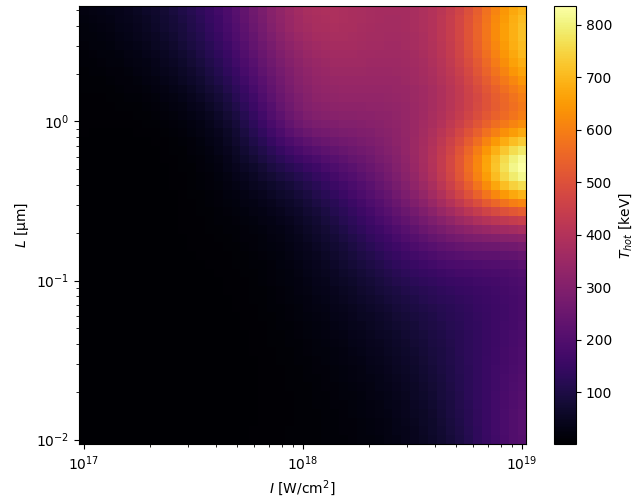
\includegraphics[width=\textwidth]{figures/improved-model}
		\caption{Temperature predictions.}
		\label{fig:gp-improved-pred}
	\end{subfigure}
	\hfill
	\begin{subfigure}{0.49\textwidth}
		\centering
		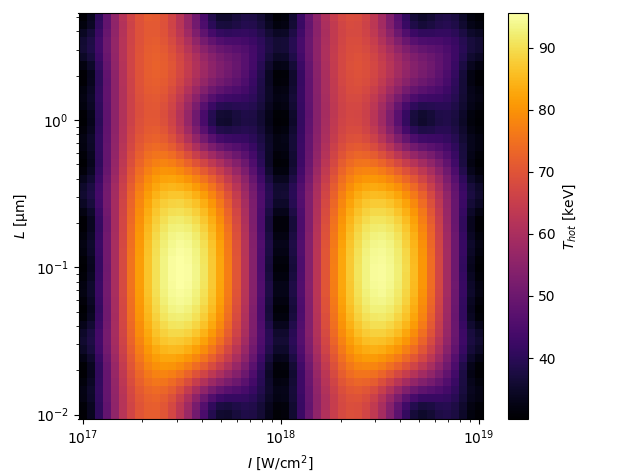
\includegraphics[width=\textwidth]{figures/improved-model-ss}
		\caption{Uncertainty (standard error estimate).}
		\label{fig:gp-improved-ss}
	\end{subfigure}
	\caption{Predictinos of the GP model for $\alpha = 0$ trained with the expanded dataset.}
	\label{fig:gp-improved}
\end{figure}

In Figure \ref{fig:gp-improved} one can see the predictions of the updated GP model. The predictions have slightly changed compared to Figures \ref{fig:graph-tool2} and \ref{fig:graph-tool3}. Both predictions and the uncertainties are lower where the new data is. The fact that the temperatures were for some parameters overestimated might have contributed to bigger values of RMSE in the K-fold. We would need much more new simulations to reduce the uncertainty globally but let us have two final remarks to the dataset expansion.

This strategy is very similar to the intuitive approach where we add point to regions with few points. However, neither this nor our strategy is including the information about the shape of the predictions. If the number of new simulations is small, one should select the regions that are particularly interesting to him after examining the predictions visually. The idea is, that where the temperature is changing more steeply, the smoothening might not be as useful as elsewhere. The error introduced by too strict smoothening can be reduced by new data in steep regions.

Let us not forget, that all of the models we used are regression models and they can sometimes treat the maximum values of dataset to be outliers. This can also be compensated for example with improving the dataset density in regions with highest predictions.